\documentclass[twoside=false, %  doppelseitiger Druck
DIV=15,% DIV Faktor für Satzspiegelberechnung, sie Doku zu KOMA Script
BCOR=15mm, % Bindekorrektur
chapterprefix=false,
headinclude=true,
footinclude=false,
pagesize,%         write pagesize to DVI or PDF
fontsize=11pt,%             use this font size
paper=a4,%          use ISO A4
bibliography=totoc,%         write bibliography-chapter to table of contents
index=totoc,%         write index-chapter to table of contents
cleardoublepage=plain,% \cleardoublepage generates pages with pagestyle empty
headings=big,%       A4/B5
listof=flat,%        improved list of tables
numbers=noenddot
]{scrbook}
\usepackage{listings}

\addtokomafont{chapter}{\normalfont\bfseries}
\addtokomafont{section}{\normalfont\bfseries}
\addtokomafont{subsection}{\normalfont\bfseries}
\addtokomafont{caption}{\small}

\usepackage{amsmath}
\usepackage[linesnumbered,ruled]{algorithm2e}

%theorems and shaded
\usepackage{framed}
\usepackage{amsthm}
\usepackage{thmtools}
\theoremstyle{definition}
\newtheorem{mythm}{Definition}

\usepackage[dvipsnames]{xcolor}
\lstdefinestyle{fsharpStyle}{
  language=fsharp,
  basicstyle=\ttfamily,
  commentstyle=\itshape\color{gray},
  keywordstyle=\bfseries\color{blue},
  numbers=left,
  numberstyle=\tiny\color{gray},
  frame=none,
  breaklines=true,
  showstringspaces=false
}
\colorlet{punct}{red!60!black}
\definecolor{background}{HTML}{EEEEEE}
\definecolor{delim}{RGB}{20,105,176}
\colorlet{numb}{magenta!60!black}
\lstdefinelanguage{json}{
    basicstyle=\normalfont\ttfamily,
    numbers=left,
    numberstyle=\scriptsize,
    stepnumber=1,
    numbersep=8pt,
    showstringspaces=false,
    breaklines=true,
    frame=lines,
    backgroundcolor=\color{background},
    literate=
     *{0}{{{\color{numb}0}}}{1}
      {1}{{{\color{numb}1}}}{1}
      {2}{{{\color{numb}2}}}{1}
      {3}{{{\color{numb}3}}}{1}
      {4}{{{\color{numb}4}}}{1}
      {5}{{{\color{numb}5}}}{1}
      {6}{{{\color{numb}6}}}{1}
      {7}{{{\color{numb}7}}}{1}
      {8}{{{\color{numb}8}}}{1}
      {9}{{{\color{numb}9}}}{1}
      {:}{{{\color{punct}{:}}}}{1}
      {,}{{{\color{punct}{,}}}}{1}
      {\{}{{{\color{delim}{\{}}}}{1}
      {\}}{{{\color{delim}{\}}}}}{1}
      {[}{{{\color{delim}{[}}}}{1}
      {]}{{{\color{delim}{]}}}}{1},
}

\usepackage{geometry}
\usepackage{array}
\usepackage{acronym}
\usepackage[utf8]{inputenc}
\usepackage{makeidx}
%\usepackage{amsfonts}
%\usepackage[slantedGreek,sc]{mathpazo}  % Schriftart Palatino
% \usepackage{lmodern}    % statt mathpazo, falls CM Fonts verwendet werden sollen
%\usepackage{mathptmx}    % statt mathpazo, falls Times  verwendet werden soll
\usepackage[scaled=.95]{helvet}
\usepackage{courier}
\usepackage[T1]{fontenc}
\usepackage{textcomp}
\usepackage{amsmath}            % standard math notation (vectors/sets/...)
\usepackage{bm}        % standard math notation (fonts)
\usepackage{fixmath}        % standard math notation (fonts)
\usepackage{graphicx}
\usepackage[facing=yes]{floatrow}       % mehrere Gleitobjekte nebeneinander/caption neben Bild/Tabelle
\usepackage[labelfont=bf,sf,font=small,labelsep=space,format=plain]{caption}
\usepackage{subcaption}
\usepackage{scrlayer-scrpage}
% \usepackage{pstool}  % einbinden falls psfrag verwendet werden soll
\usepackage{epstopdf}
\usepackage[english]{babel}
\usepackage{ellipsis}  % Korrigiert den Weißraum um Auslassungspunkte
\usepackage{microtype}  % optischer Randausgleich etc.

\usepackage{xcolor}         % z.B. für schattierte Boxen
\usepackage{framed}			% shaded Umgebung
\definecolor{shadecolor}{gray}{.85}%

% Links im PDF
\usepackage[colorlinks=false,
        pdfborder={0 0 0},
        breaklinks=true]
        {hyperref}


%\typearea[current]{calc}


% Einstellungen für Bild-/Tabellenbeschriftung neben dem Bild
\floatsetup[figure]{capbesideposition={inside,top}}
\floatsetup[table]{capbesideposition={inside,top},style=plaintop}
\renewfloatcommand{fcapside}{figure}[\capbeside][\FBwidth]
\newfloatcommand{tcapside}{table}[\capbeside][\FBwidth]


\selectlanguage{english}


\deffootnote{1em}{1em}{%
\makebox[1em][l]{\thefootnotemark}}

\makeindex

\newcommand{\real}{\mathord{\mathrm{I\!R}}}

\begin{document}
\selectlanguage{english}
\def\figdir{figures}
%\def\tabledir{tables}

\frontmatter

\pagestyle{scrplain}
\pagestyle{empty}

\begin{titlepage}

%\sffamily

\raggedleft

\vspace*{-2cm}


\includegraphics{logo-th-rosenheim-2019_master_quer_2c.eps}

\vfill

\centering
\LARGE
% \vspace*{\fill}
%-----------
Department of Computer Science  \vspace{0.5cm}\\
\Large
Master Computer Science

\vspace{2cm}

\LARGE

NerdDeck --- A comparison of functional programming paradigms between Go and Haskell

\vspace{2cm}

\Large
Course work in \textit{Concepts of programming langugages}\vspace{0.5cm}\\
Winter term 2023/2024

\vspace{1.5cm}


\Large
from

\vspace{0.5cm}

%\vspace*{\fill}

\LARGE
Maximilian Gobbel \vspace{0cm}

%\today

\vspace{1cm}

\flushleft
 \Large
\vspace*{\fill}


\end{titlepage}

\cleardoubleemptypage

{
\large
\thispagestyle{empty}
\vspace*{\fill}

\noindent
\textsc{Declaration of Originality}

\medskip

\noindent
I declare that I have authored this thesis independently, that I have not used other than the declared sources / resources, and that I have explicitly marked all material which has been quoted either literally or by content from the used sources.

\bigskip

\noindent
Rosenheim, \today

\vspace*{2cm}

\noindent
Maximilian Gobbel
}

%%% Local Variables: 
%%% mode: latex
%%% TeX-master: "d"
%%% End: 

\cleardoubleemptypage
\chapter*{Abstract}
\thispagestyle{empty}


\bigskip

\noindent
Keywords: Go, Haskell, Functional Programming, Comparison


\cleardoubleemptypage

\pagestyle{scrplain}
\pagenumbering{roman}
\tableofcontents
\clearpage
\listoffigures
\clearpage
\listoftables
\cleardoublepage


\pagestyle{scrheadings}


\addtokomafont{caption}{\small}

\mainmatter

\chapter{Introduction}\label{chap:introduction}
This paper is written for the master course \textit{Concepts of Programming Languages} of the apartment of computer science in the Winter Term 23/24 at the Technical University of Applied Sciences Rosenheim.
    \section{Background}\label{sec:background}
As of the TIOBE Index data as of November 2023, it is reported that there are currently over 150 programming languages in existence. This implies that, up until the present moment, the programming landscape continues to encompass a diverse array of languages, reflecting the dynamic and ever-evolving nature of the field.\cite{tiobeindex} The task of a programmer at a certain point in the production of software is to select one of these programming languages that is suitable for a particular problem. This can be a science in itself. This very topic has been discussed for around 50 years.\cite{Tharp1982}
The reason for that is that every language has its own paradigms and concepts. One can come up with a solution, selecting a language which fits a lot of problems but not a single one perfect. Or he selects one which fits perfect for a single problem but it is not possible to solve all the other problems.
So the goal would be to select the \textit{right} programming language which suits the requirements and the surrounding of a given problem accordingly.
This spot should be covered by this paper with the comparison of Go and F\# in the context of \ac{fp}.

    \section{Purpose of the Project}\label{sec:purpose}
    The primary objective of this project is to analyse and explore the distinction and similarities between two languages within the realm of \ac{fp}. The selected languages for this comparative study are Go\footnote{Website: \url{https://go.dev} (Accessed on 12/02/2023)} and F\#\footnote{Website: \url{https://dotnet.microsoft.com/languages/fsharp} (Accessed on 12/02/2023)}. Go was chosen as the initial language due to its consistent usage throughout the course, making it mandatory inclusion in the project. 
    In addition to Go, a second programming language is essential for the comparative analysis, and F\# has been selected for this purpose. The decision to include F\# in this study is based on the author's deliberate choice, and the relationale behind this decision is elucidated in the subsequent section \ref{sec:whyfsharp}. By juxtaposing Go and F\#, the project aims to unravel the nuances and divergences in their approaches to \ac{fp} paradigms, shedding light on their distinctive features, strengths, and potential use cases. Through this comparative exploration, the project seeks to contribute valuable insights into the \ac{fp} landscape, providing a nuanced understanding of the strengths and trade-offs associated with these two languages.

    \section{Why F\#?}\label{sec:whyfsharp}
    One of the key reasons for choosing F\# is its status as a functional-first programming language. In contrast to Go's multi-paradigm approach, F\#'s commitment to functional principles provides an excellent opportunity to explore the benefits of implementing code from a pure perspective.
    For a more in-depth understanding of F\#, including its syntax, features, and \ac{fp} principles, readers are encouraged to refer to section \ref{sec:fsharp-overview}.

    \section{Roadmap}\label{sec:roadmap}
    Embedded within this exploration about \ac{fp} is a brief discussion of the \textit{NerdDeck} Flash Card \ac{app} in chapter 2, our practical context for understanding \ac{fp} in action. Besides of that this paper navigates a concise roadmap to compare \ac{fp} in Go and F\#, anchored by an initial overview of \ac{fp} principles in chapter 3. It then swiftly transitions to individual language analyses in chapter 4, spotlighting key design philosophies and features of Go and F\#. The centerpiece is chapter 5, a focused exploration of two critical functional concepts: Algebraic Data Types and Pattern Matching. Leveraging code examples, this section illuminates nuances in implementation, providing a succinct yet insightful comparative analysis. The paper concludes in chapter 6, summarizing challenges, key findings, and lessons learned from both the project and the comparative analysis. This streamlined roadmap ensures a comprehensive yet condensed examination of \ac{fp} in Go and F\#.

\chapter{Project Overview}\label{chap:project-overview}
    \section{Description of the \textit{NerdDeck} Flash Card Application}\label{sec:description}
    \textit{NerdDeck} is app which can help remembering things with flashcards. There exists already such a product called Anki\footnote{Website: \url{https://apps.ankiweb.net} (Accessed on 12/03/2023)} for the same usecase. Most parts of Anki are written in Rust and Python.\footnote{Website: \url{https://github.com/ankitects/anki} (Accessed on 12/03/2023)} The difference in \textit{NerdDeck} is that is written twice, each time in a different programming language, Go and F\#, and the \ac{fp} paradigma should be used. In F\# there will be no problem as it will turn out in section \ref{sec:fsharp-overview} because it is possible to write pure code. But as Go is a impure language, the goal is to write it as functional as possible. In addition to that, \textit{NerdDeck} should just use the \ac{cli} as a \ac{gui} while Anki has a own one.

    \section{Requirements}
    The coding project should illustrate and highlight similarities and differences about \ac{fp}. The \ac{app} should allow a single user to use the \ac{sm2} alorithm which is used for spaced repetition.\cite{sm2} One of Anki's algroithms is also based on \ac{sm2}.\footnote{Website: \url{https://faqs.ankiweb.net/what-spaced-repetition-algorithm.html} (Accessed on 12/03/2023)} Because \textit{NerdDeck} is build by a student, the requirements are also written from a students perspective. The requirements are written down in table \ref{tab:requirements}. These should not differ too big from other users using this application. The program should act as a \ac{mvp}, so it's possible to do the comparison about \ac{fp}. The goal is to implement this twice, one time in Go and then in F\#, both in a functional style.
    \begin{table}[h]
        \centering
        \begin{tabular}{|m{0.5in}|m{4in}|}
            \hline
            \textbf{ID} & \textbf{Requirement} \\
            \hline
            1 & As a student, I want to create a flashcard. \\
            \hline
            2 & As a student, I want to create a deck of flashcards. \\
            \hline
            3 & As a student, I want to assign a flashcard to a deck. \\
            \hline
            4 & As a student, I want to be able to create multiple decks. \\
            \hline
            5 & As a student, I want to view my flashcards. \\
            \hline
            6 & As a student, I want to delete my flashcards. \\
            \hline
            7 & As a student, I want to apply spaced repetition. \\
            \hline
        \end{tabular}
        \caption{\textit{NerdDeck} Requirements}
        \label{tab:requirements}
    \end{table}

    \section{Data}
    For the purpose of this project, a single \ac{json} file is used as a simple and lightweight database to store flashcards. While this approach is suitable for educational and illustrative purposes, it may not be suitable for production usage due to limitations in scalability and concurrent access. In a production environment, a more robust database solution should be considered, such as a relational database (e.g., PostgreSQL\footnote{Website: \url{https://www.postgresql.org} (Accessed on 12/02/2023)}, MySQL\footnote{Website: \url{https://www.mysql.com} (Accessed on 12/02/2023)}) or a NoSQL database (e.g., MongoDB\footnote{Website: \url{https://www.mongodb.com} (Accessed on 12/02/2023)}). The choice of the database will depend on the specific requirements of the \ac{app}.

    \subsection{Model}
    To be able to the requirements of table \ref{tab:requirements} a model is needed for both a flashcard and also for a deck. These are shown in figure \ref{fig:er-model}. It is important that a deck can contain multiple flashcards while a flashcard always remains to a single deck. This model should be used within both languages.

    \begin{figure}
        \centering
        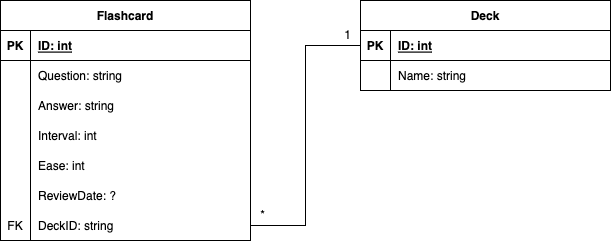
\includegraphics[width=1\textwidth]{NerddeckModel.png}
        \caption{Entity-Relationship Model of Flashcard and Deck}
        \label{fig:er-model}
    \end{figure}

    \begin{lstlisting}[language=json,firstnumber=1,float=tp, caption={Example of how a flashcard is saved inside a \ac{json} file}, label=l:flashcardjson]
    [
    {
        "Question": "What is functional programming?",
        "Answer": "Functional programming is a programming paradigm that treats computation as the evaluation of mathematical functions and avoids changing-state and mutable data.",
        "Interval": 1,
        "Ease": 1,
        "ReviewDate: ?,
        "DeckID: ""
    }
    ]
        
    \end{lstlisting}


    \chapter{Overview of functional programming}\label{chap:functional-programming}
    \begin{shaded}
        \noindent
        \glqq{}As software becomes more and more complex, it is more and more important to structure it well. Well-structured software is easy to write, easy to debug, and provides a collection of modules that can be re-used to reduce future programming costs. Conventional languages place conceptual limits on the way problems can be modularised. Functional languages push those limits back.\grqq{} \cite{Hughes1989}
    \end{shaded}
    This should be the motivation considering the usage of \ac{fp}.
    Within the paradigm of \ac{fp}, developers engage with principles that underscore the pursuit of expressive and concise solutions. Rooted in mathematical concepts like lambda calculus, \ac{fp} emerges as a methodology characterized by rigor and elegance.
    
    Key principles integral to \ac{fp} include:
    
    \begin{itemize}
        \item \textbf{Purity:} Strict avoidance of side effects to ensure deterministic behavior.
        \item \textbf{Higher-order functions:} Utilization of functions as parameters and return values for enhanced modularity.
        \item \textbf{Lazy evaluation:} Selective computation, evaluating values only when necessary for optimization.
        \item \textbf{Algebraic data types:} Incorporation of sum- and product-types, as discussed in more detail in Section \ref{sec:algebraic-data-types}.
        \item \textbf{Pattern Matching:} A powerful technique, elaborated further in Section \ref{sec:pattern-matching}.
    \end{itemize}
    
    Originating in 1950 with the introduction of the impure language LISP, \ac{fp} has evolved across languages like F\# and Go. F\# strictly adheres to a pure functional approach, emphasizing immutability and mathematical principles, while Go incorporates impure functional elements, showcasing the adaptability of \ac{fp} principles. Additional insights into this topic are expounded upon in Chapter \ref{chap:language-comparison}.
    
    As developers navigate through contrasting algorithms, exploring the interplay between imperative and declarative styles, they reflect on the historical evolution and diversity of \ac{fp} languages. This exploration serves as a testament to the flexibility of programming paradigms and prompts consideration of the nuanced trade-offs between explicit instruction and expressive abstraction within the dynamic context of \ac{fp}.
    
    In conclusion, \ac{fp} equips professionals with a robust set of tools, emphasizing immutability, higher-order functions, and mathematical principles. It not only addresses contemporary challenges in software development but also fosters a deeper understanding of the intricacies involved in designing robust, modular, and expressive code.
    

\section{Imperative vs. Declarative}

Within the broader spectrum of programming paradigms, the imperative and declarative styles represent two contrasting approaches to articulating code. In the following the two approaches will be shown on a simple algorithm: summing up a array of numbers.

\subsubsection{Imperative Approach}

The imperative paradigm, exemplified by Algorithm \ref{alg:imperative_sum}, guides the computer through computations using explicit steps. Each line of pseudocode instructs the computer on how to perform the calculation, adhering to traditional imperative paradigms.

\begin{algorithm}
    \SetKwInOut{Input}{Input}
    \SetKwInOut{Output}{Output}

    \underline{function SumArray} $(a)$\;
    \Input{Integer Array $a$}
    \Output{Sum of elements in $a$}
    
    \BlankLine
    $result \leftarrow 0$
    
    \ForEach{$element$ \textbf{in} $a$}
    {
        $result \leftarrow result + element$
    }
    
    \Return $result$
    
    \caption{Imperative way of summing up an integer array}
    \label{alg:imperative_sum}
\end{algorithm}

\subsubsection{Declarative Approach}

In contrast, the declarative style, showcased by Algorithm \ref{alg:declarative_sum}, shifts the emphasis from detailing step-by-step procedures to expressing the desired outcome directly. This approach, a hallmark of \ac{fp}, leverages the power of functions and abstraction.

\begin{algorithm}
    \SetKwInOut{Input}{Input}
    \SetKwInOut{Output}{Output}

    \underline{function SumArray} $(a)$\;
    \Input{Integer Array $a$}
    \Output{Sum of elements in $a$}
    
    \BlankLine
    \Return $\sum_{\text{element in } a} \text{element}$
    
    \caption{Declarative way of summing up an integer array}
    \label{alg:declarative_sum}
\end{algorithm}

The juxtaposition of these algorithms not only highlights the difference in coding philosophy but also serves as a tangible exploration of the imperative and declarative styles within the context of \ac{fp}.


\chapter{Introduction to Go and F\#}\label{chap:language-comparison}
In this chapter, we delve into the distinctive features of Go and F\#, offering a brief overview of each language before embarking on comparative analysis.

    \section{Overview of Go}\label{sec:go-overview}
    The usage of the programming language Go allows to build simple, secure and scalable systems. It is used very widely within big companys like Google, Paypal or Netflix. Besides of that it is open source. \cite{GoWebsite}
    \section{Overview of F\#}\label{sec:fsharp-overview}
    F\# is a functional-first programming language
    Besides C\# and Visual Basic, F\# is third programming language within the .NET ecosystem. On the official website of microsoft it is delared as an open-source language that makes it easy to write succinct, robust, and performant code. Microsoft names itself as a leading contributor. Because F\# is part of the .NET system of microsoft it offers a lot of advantages like the interoperability with the other languages. This means it is easy to execute C\# code from F\# code and vice verca. It is also possible to access .NET Libraries and APIs (e.g. ASP.NET or Entity Framework). F\# has an active community and support. While developing, F\# has a very powerful build-in future called \ac{repl}.
\cite{dotnet}
f
\chapter{Comparison of functional concepts}
In order to compare the two languages, the following two functional concepts are examined in more detail: Algebraic Data Types and Pattern Matching. Both of the languages are not completely pure like for example Haskell\footnote{Website: \url{https://www.haskell.org} (Accessed on 12/20/2023)}.
    \section{Algebraic Data Types}\label{sec:algebraic-data-types}
    In F\# there are two types of algebraic data types: record types and discriminated unions. In Nerddeck a record type is used to model a flashcard and the flashcard deck. 
    \section{Pattern Matching}\label{sec:pattern-matching}
    Pattern Matching works perfectly when you already have algebraic data types inside your programming language.


\chapter{Conclusion}\label{chap:conclusion}
    \section{Challenges}\label{sec:challenges}
    The foundation of a good comparision in the context of this paper is to write code as pure as possible to fulfill the paradigm of functional programming. Since Go and also F\# is not completely pure...
    \section{Summary of Findings}\label{sec:findings-summary}
    \section{Lessons Learned}\label{sec:lessons-learned}




\appendix
\include{append}
\chapter{Appendix}

\chapter*{Acronyms}

\begin{acronym}

    \acro{app}[App]{Application}
    \acro{cli}[CLI]{Command Line Interface}
    \acro{fp}[FP]{functional programming}
    \acro{gui}[GUI]{Graphical User Interface}
    \acro{json}[JSON]{JavaScript Object Notation}
    \acro{mvp}[MVP]{Minimal Viable Product}
    \acro{repl}[REPL]{Read-eval-print loop}
    \acro{sm2}[SM2]{SuperMemo 2.0}
    \acro{uml}[UML]{Unified Modeling Language}

\end{acronym}

\listoffigures{}
\lstlistoflistings{}
\listoftables{}

\cleardoublepage

\bibliographystyle{natger}
\bibliography{document}

\cleardoublepage


\footnotesize
\printindex

\end{document}